\chapter{Simulation Environments and Input Data}
\label{sec:simulation_environments_and_data}

LodusPop is designed to model simulation scenarios using real-world spatial, demographic, and service data. To evaluate this capability in an urban setting, we model the city of Porto Alegre and its population using three main representations. The first represents both population and points of interest (POIs) at the neighborhood level. The second preserves neighborhoods as simulation regions while representing population and POIs at the finer census-sector level across the entire city. The third uses the same census-sector-level representation but is restricted to 13 neighborhoods in the central area of Porto Alegre. 

In addition to environment and population data, service, flood, shelter, and behavioral datasets are overlaid on the representation appropriate to each use case. This chapter presents these environments and their shared inputs, distinguishing between observed or externally sourced data, data derived through spatial or statistical preprocessing, and values configured specifically for each simulation scenario.

Following the definitions introduced in Chapter~\ref{chapter:proposed_model}, each input described in this chapter has one of two roles. Core inputs initialize point-of-interest types and attributes, population blobs and their characteristics, or local and global routines. Experiment-specific inputs instead configure plugins through $\bm{\theta}_{\Pi}$, extend the model vocabulary through $\Delta\Sigma_{\Pi}$, or provide data used by routine contributions, action handlers, and lifecycle hooks. This distinction separates the provenance of an input from the mechanism through which it affects the simulation.


\section{Spatial Representations}
\label{sec:spatial_population_environments}

Following the environment definition introduced in Section~\ref{sec:environment}, neighborhoods are modeled as simulation regions ($R$), each containing a set of points of interest ($P$). The environments differ primarily in their spatial extent and in the resolution at which population and POIs are represented.




\subsection{Neighborhood-Level Environment}

The neighborhood-level Porto Alegre model follows the environment described in the published LodusPop manuscript~\cite{silva2026lodusPop}. Each of the city's 94 neighborhoods is represented as a simulation region. Neighborhood boundaries were obtained from digital cartographic data published by Porto Alegre City Hall\footnote{Porto Alegre City Hall digital maps, including the neighborhood boundary layer (``Bairros (LC 12.112/16)''): \url{https://prefeitura.poa.br/carta-de-servicos/mapas-digitais-da-smamus}.}, while OpenStreetMap was used to obtain coordinates for urban amenities represented as POIs\footnote{OpenStreetMap: \url{https://www.openstreetmap.org/}.}. Each region contains one POI of each standard type $\tau_i$: \textit{home}, \textit{work}, \textit{school}, \textit{marketplace}, \textit{pharmacy}, and \textit{gas station}.
Selected regions also contain POIs with specialized types, such as shopping malls and stadiums, when required by an experiment. Coordinates, external identifiers, and other location-specific values are stored in the POI attribute mapping $\bm{\alpha}_i$.


Population totals, citywide occupation proportions, and the citywide age distribution were obtained from the 2010 Census of the Brazilian Institute of Geography and Statistics (IBGE)\footnote{IBGE city profile for Porto Alegre: \url{https://cidades.ibge.gov.br/brasil/rs/porto-alegre/panorama}.}. Neighborhood-level population and age distributions were complemented with municipal information published by ObservaPOA and PROCEMPA\footnote{ObservaPOA: \url{http://www.observapoa.com.br/}. PROCEMPA's Porto Alegre em Análise portal: \url{https://portoalegreemanalise.procempa.com.br/}.}.


One initial population blob is placed at the home POI of each neighborhood. Age and occupation are represented as sampled characteristics in $\bm{Sc}$ because each blob stores a distribution over their categories. Traceable characteristics required by a particular experiment, such as infection, vaccination, mobility-lifecycle, or patient states, are subsequently declared with defaults by the corresponding plugin through $\Delta\Sigma_{\Pi}$.

Occupation is divided into \textit{students}, \textit{workers}, and \textit{others}. Because neighborhood-level occupation distributions were unavailable, the same citywide distribution was applied to every neighborhood: approximately 21.6\% students, 54.7\% workers, and 23.7\% others. 


Age is divided into four categories: \textit{child} (0--14 years), \textit{young} (15--24 years), \textit{adult} (25--59 years), and \textit{elder} (60+ years). Each neighborhood uses its corresponding age distribution, while the overall modeled population consists of approximately 18.7\% children, 15.7\% young people, 50.5\% adults, and 15.1\% elders. Overall, the neighborhood-level environment comprises 94 regions ($R$), 504 POIs ($P$), and a total population of 1,409,351.

\subsection{Census-Sector-Level Environments}

The more detailed environments use census sectors, also referred to as enumeration areas, as the spatial unit for population initialization. Neighborhoods remain the simulation regions, preserving compatibility with region-level routines and outputs, while census sectors provide a finer spatial representation of the population and associated POIs. Official census-sector aggregates and geographic files were obtained from the 2022 IBGE Census\footnote{IBGE 2022 Census sectors: \url{https://www.ibge.gov.br/geociencias/organizacao-do-territorio/malhas-territoriais/26565-malhas-de-setores-censitarios-divisoes-intramunicipais.html}.}.

The neighborhood-level environment described in the previous section was originally constructed using demographic data from the 2010 IBGE Census, consistent with the environment used in the published LodusPop experiments. The census-sector environments were subsequently constructed using the more recent 2022 Census data. %Consequently, differences in population totals between these environments reflect both their spatial representation and the underlying census datasets.


In both census-sector environments, six standard POIs are instantiated for each census sector within the neighborhood region containing that sector. Their types correspond to \textit{home}, \textit{work}, \textit{school}, \textit{marketplace}, \textit{pharmacy}, and \textit{restaurant}. The census sector is therefore the unit used to position and initialize these POIs, whereas the neighborhood remains the simulation region $R$. The population associated with each sector is initially represented by a blob at its corresponding home POI.

We consider two versions of this representation: a \textit{complete environment}, covering all 94 neighborhoods of Porto Alegre, and a \textit{reduced environment}, restricted to 13 neighborhoods in the central area of the city.
The complete environment applies this representation to 2,711 census sectors distributed across all 94 neighborhoods, resulting in 16,266 POIs and a total population of 1,331,414. The reduced environment applies the same representation to 435 census sectors distributed across 13 central neighborhoods, resulting in 2,610 POIs and a total population of 159,886.

Table~\ref{tbl:shared_simulation_environments} summarizes the three environment versions. Figure~\ref{fig:spatial_representations} presents their spatial representations, highlighting the distribution of home POIs.




\begin{table}[ht]
\centering
\footnotesize
\setlength{\tabcolsep}{4pt}
\caption{Porto Alegre environments used by the result sections.}
\label{tbl:shared_simulation_environments}
\begin{tabularx}{\linewidth}{@{}p{2.6cm}rrrrX@{}}
\toprule
\textbf{Environment} &
\textbf{Regions} &
\textbf{Home POIs} &
\textbf{Total POIs} &
\textbf{Population} &
\textbf{Main use cases} \\
\midrule
Neighborhood-level
    & 94 & 94 & 504 & 1,409,351
    & Published L\'evy Walk, large-scale events, epidemic contagion, and vaccination. \\
Reduced census-sector
    & 13 & 435 & 2,610
    & 159,886
    & Popular Times, L\'evy Walk, dialysis, and flood-aware mobility. \\
Complete census-sector, 
    & 94 & 2,711 & 16,266
    & 1,331,414
    & Popular Times, L\'evy Walk, dialysis, and flood-aware mobility. \\
\bottomrule
\end{tabularx}
\end{table}

\begin{figure}[ht]
 \centering
  
\includegraphics[width=0.99\textwidth]{fig/viz/spatial_environment_comparison.png}
  \caption{Spatial representations of Porto Alegre.} 
  \label{fig:spatial_representations}
\end{figure}


\section{Scenario-Specific Experimental Inputs}
\label{sec:scenario_specific_inputs}

The shared spatial representations are extended with additional inputs according to the phenomenon examined by each experiment. To facilitate the connection between these inputs and the corresponding results, they are presented in the same order as in the experimental-results chapter: routine mobility; large-scale events, contagion, and vaccination; environmental disruptions; and health services.

Table~\ref{tbl:input_plugin_mapping} connects these input families to the extension contract defined in Section~\ref{sec:plugins}. The mapping identifies the principal nonempty components used by each experiment family; individual experimental sections report the selected parameter values and policies in greater detail. Environment fields such as $\tau_i$, $\bm{\alpha}_i$, $C_i(t)$, and $D_i$ remain part of the core simulation state even when a plugin declares their conventions or modifies their values.

\begin{table}[ht]
\color{red}
\centering
\footnotesize
\setlength{\tabcolsep}{4pt}
\caption{Principal mapping from scenario-input families to the plugin extension contract.}
\label{tbl:input_plugin_mapping}
\begin{tabularx}{\linewidth}{@{}p{3.0cm}p{3.4cm}X@{}}
\toprule
\textbf{Experiment family} & \textbf{Principal components} & \textbf{Role of the inputs} \\
\midrule
Routine mobility
& $\bm{\theta}_{\Pi}$, $\Delta\Sigma_{\Pi}$, $\mathcal{F}_{\Pi}$, $\mathcal{H}_{\Pi}$
& Configures mobility distributions or temporal profiles, declares lifecycle characteristics, and supplies the handlers and step updates that generate and consume movement requests. \\
Large-scale events
& $\bm{\theta}_{\Pi}$, $\mathcal{R}_{\Pi}$, $\mathcal{F}_{\Pi}$
& Defines event times and demand volumes, schedules gathering requests, and consumes them through registered action handlers. \\
Contagion and vaccination
& $\bm{\theta}_{\Pi}$, $\Delta\Sigma_{\Pi}$, $\mathcal{F}_{\Pi}$, $\mathcal{H}_{\Pi}$
& Defines epidemiological and vaccination parameters, declares population states, and updates those states during execution. \\
Flooding and shelters
& $\bm{\theta}_{\Pi}$, $\Delta\Sigma_{\Pi}$, $\mathcal{F}_{\Pi}$, $\mathcal{H}_{\Pi}$
& Provides hazard and capacity parameters, declares POI-attribute conventions and population states, and implements availability and displacement policies. \\
Dialysis services
& $\bm{\theta}_{\Pi}$, $\Delta\Sigma_{\Pi}$, $\mathcal{F}_{\Pi}$, $\mathcal{H}_{\Pi}$
& Configures recurring demand, clinic schedules and capacity, declares patient states, and implements treatment and return transitions. Clinic dependencies remain represented by $D_i$. \\
\bottomrule
\end{tabularx}
\end{table}

\subsection{Routine Mobility Inputs}
\label{sec:behavioral_policy_input_data}

The routine-mobility experiments establish baseline movement patterns that are subsequently modified by events, environmental disruptions, and service-specific demands. Two mobility configurations are considered: a stochastic L\'evy Walk model and routines driven by temporal activity profiles.


\paragraph{L\'evy Walk.}
The L\'evy Walk experiments evaluate mobility generated from configurable behavioral rules and controlled changes to routine activity. Their configurations add behavioral parameters rather than observed trajectories. These include the heavy-tailed distance scale, packet size, restriction factor, worker attendance rate, student attendance rate, departure-hour profiles, and visit durations. Their role is to define internally consistent baseline behaviors and controlled comparisons. %Unless supported by a cited calibration dataset, they should not be interpreted as estimates of Porto Alegre's realized commuting patterns.
These values form the mobility plugin configuration $\bm{\theta}_{\Pi}$. The plugin declares the traceable characteristics needed to follow commute lifecycles through $\Delta\Sigma_{\Pi}$ and registers the handlers and step updates in $\mathcal{F}_{\Pi}$ and $\mathcal{H}_{\Pi}$. The resulting movement requests retain the common action structure $A=(N,T,\bm{V})$, with templates distinguishing worker and student populations.


\paragraph{Popular Times.}
The Popular Times experiments evaluate routine mobility generated from time-varying demand for different types of urban activities. The routines use three seven-day hourly profiles, one each for marketplaces, restaurants, and pharmacies. These profiles were synthetically constructed by a colleague of the author based on the temporal patterns shown by the Popular Times feature of Google Maps. Unlike the stochastic destination and timing choices of the L\'evy Walk configurations, these profiles provide scheduled activity demand that varies according to POI type and time of day.

The profile files and visit-rate parameters form $\bm{\theta}_{\Pi}$. At each applicable simulation step, the plugin uses the simulation cycle and cycle step (i.e, current simulated day and hour) to generate requests for POIs whose type $\tau_i$ matches the profile. Its schema additions record visit lifecycles, while its action handler selects population through $T$ and applies the configured destination and return policies.


\subsection{Large-Scale Events, Contagion, and Vaccination}

These experiments extend routine mobility with temporary gathering demands and longer-term changes to population characteristics. They are used to evaluate how the same population representation can accommodate both short-lived changes in destination demand and processes that evolve across multiple simulation cycles.

\paragraph{Large-scale events.}
The large-scale-event experiments add short-lived gathering demands to ordinary mobility. Event destinations use existing modeled POIs whose coordinates originate from the OpenStreetMap-based environment. The request of 500,000 attendees per event and the event times are scenario-defined stress inputs rather than observed attendance records.

The event time, destination, and requested attendance belong to $\bm{\theta}_{\Pi}$. They are converted into scheduled gathering requests in $\mathcal{R}_{\Pi}$ and consumed through the corresponding handler in $\mathcal{F}_{\Pi}$ using population templates.

\paragraph{Contagion and vaccination.}
The contagion experiments combine mobility with infection, vaccination, and restriction parameters in the same population representation. Epidemic initialization, homogeneous infection and removal parameters, vaccine-effectiveness values, dose-start days, and restriction levels define comparative scenarios. The three reported $R_0$ values are based on studies of COVID-19 transmission in Brazil~\cite{dutra2020covidR0,deSouza2020covirR0,dutra2021covidR0}, while the daily vaccination quantities follow the 546-value Porto Alegre series obtained from the Rio Grande do Sul vaccination dashboard\footnote{Rio Grande do Sul COVID-19 vaccination dashboard: \url{https://vacina.saude.rs.gov.br/}.}. The dashboard reports doses applied by date, and the simulation distributes the daily Porto Alegre quantities among modeled regions in proportion to their populations.

The epidemiological, restriction, effectiveness, and dose-distribution values form $\bm{\theta}_{\Pi}$. Infection and vaccination states are traceable characteristics declared through $\Delta\Sigma_{\Pi}$, ensuring that actions can select them through $\bm{T_{Tc}}$ and that blobs with different states remain distinct during merging. Registered handlers and time-step hooks in $\mathcal{F}_{\Pi}$ and $\mathcal{H}_{\Pi}$ implement infection transitions and vaccination updates.

\subsection{Environmental-Disruption Inputs}

The environmental-disruption experiments examine how a common hazard can change the availability of locations, suppress or redirect routine mobility, and create demand for capacity-constrained shelters. Flood exposure is therefore represented separately from the water-level condition applied over time, allowing the same spatial environment to be evaluated under different disruption scenarios.

\subsubsection{Flood Exposure and Water-Level Scenarios}
\label{sec:flood_water_input_data}

The flood experiments combine a spatial representation of POI exposure with temporal or static water-level conditions. This separation allows flood intensity to vary between scenarios without modifying the underlying locations or their exposure thresholds.

Flood exposure is represented through the POI attribute $\bm{\alpha}_i[\mathrm{water\_level}]$. Despite the key name retained by the input format, this value is a location-specific exposure threshold rather than the water level currently applied to the simulation. The spatial thresholds were collected using the simulated ``Water Level'' map provided by Climate Central's Coastal Risk Screening Tool\footnote{Climate Central Coastal Risk Screening Tool, configured for water level above mean higher high water, contiguous inundation, and the best available elevation model: \url{https://coastal.climatecentral.org/map/12/-51.1996/-30.0653/?theme=water_level&map_type=water_level_above_mhhw&basemap=roadmap&contiguous=true&elevation_model=best_available&refresh=true&water_level=5.3&water_unit=m}.}. The latitude and longitude of each POI were inspected on the map at successive water levels. The threshold assigned to a POI is the minimum water level at which its location was shown as inundated. The resulting environment files contain thresholds from 3.0~m to 10.0~m.

The temporal or static forcing belongs to the water-level plugin configuration $\bm{\theta}_{\Pi}$. At each simulation step, the plugin compares the current forcing with $\bm{\alpha}_i[\mathrm{water\_level}]$. When the forcing reaches or exceeds the threshold, the plugin adds the named cause \textit{flood} to $C_i(t)$; when the condition no longer holds, it removes only that cause. A POI consequently remains unavailable while any other direct cause or unsatisfied dependency is present. This procedure converts the spatial flood map into a reusable POI vulnerability attribute without defining a universal mobility response: suppression, waiting, or redirection remains the policy of the action handler consuming the affected request.

The census-sector environments store a threshold for every modeled POI, allowing the same flood-cause mechanism to be applied selectively to any configured POI type $\tau_i$. The flood-aware mobility experiments use historical observations collected from a public Power BI dashboard\footnote{Historical water-level dashboard: \url{https://bit.ly/4wIpZPC}.}. The processed hourly sequence supplies the time-varying values in $\bm{\theta}_{\Pi}$ and reproduces the rise and recession of the flood. The shelter experiments instead use a static exposure overlay in which census sectors intersecting the modeled 5.30~m flood extent define 438 exposed sectors containing 186,522 residents.

Figure~\ref{fig:flood_state_visualization} illustrates the historical forcing and the corresponding spatial availability of POIs at the maximum water level represented in the sequence.

\begin{figure}[ht]
\centering
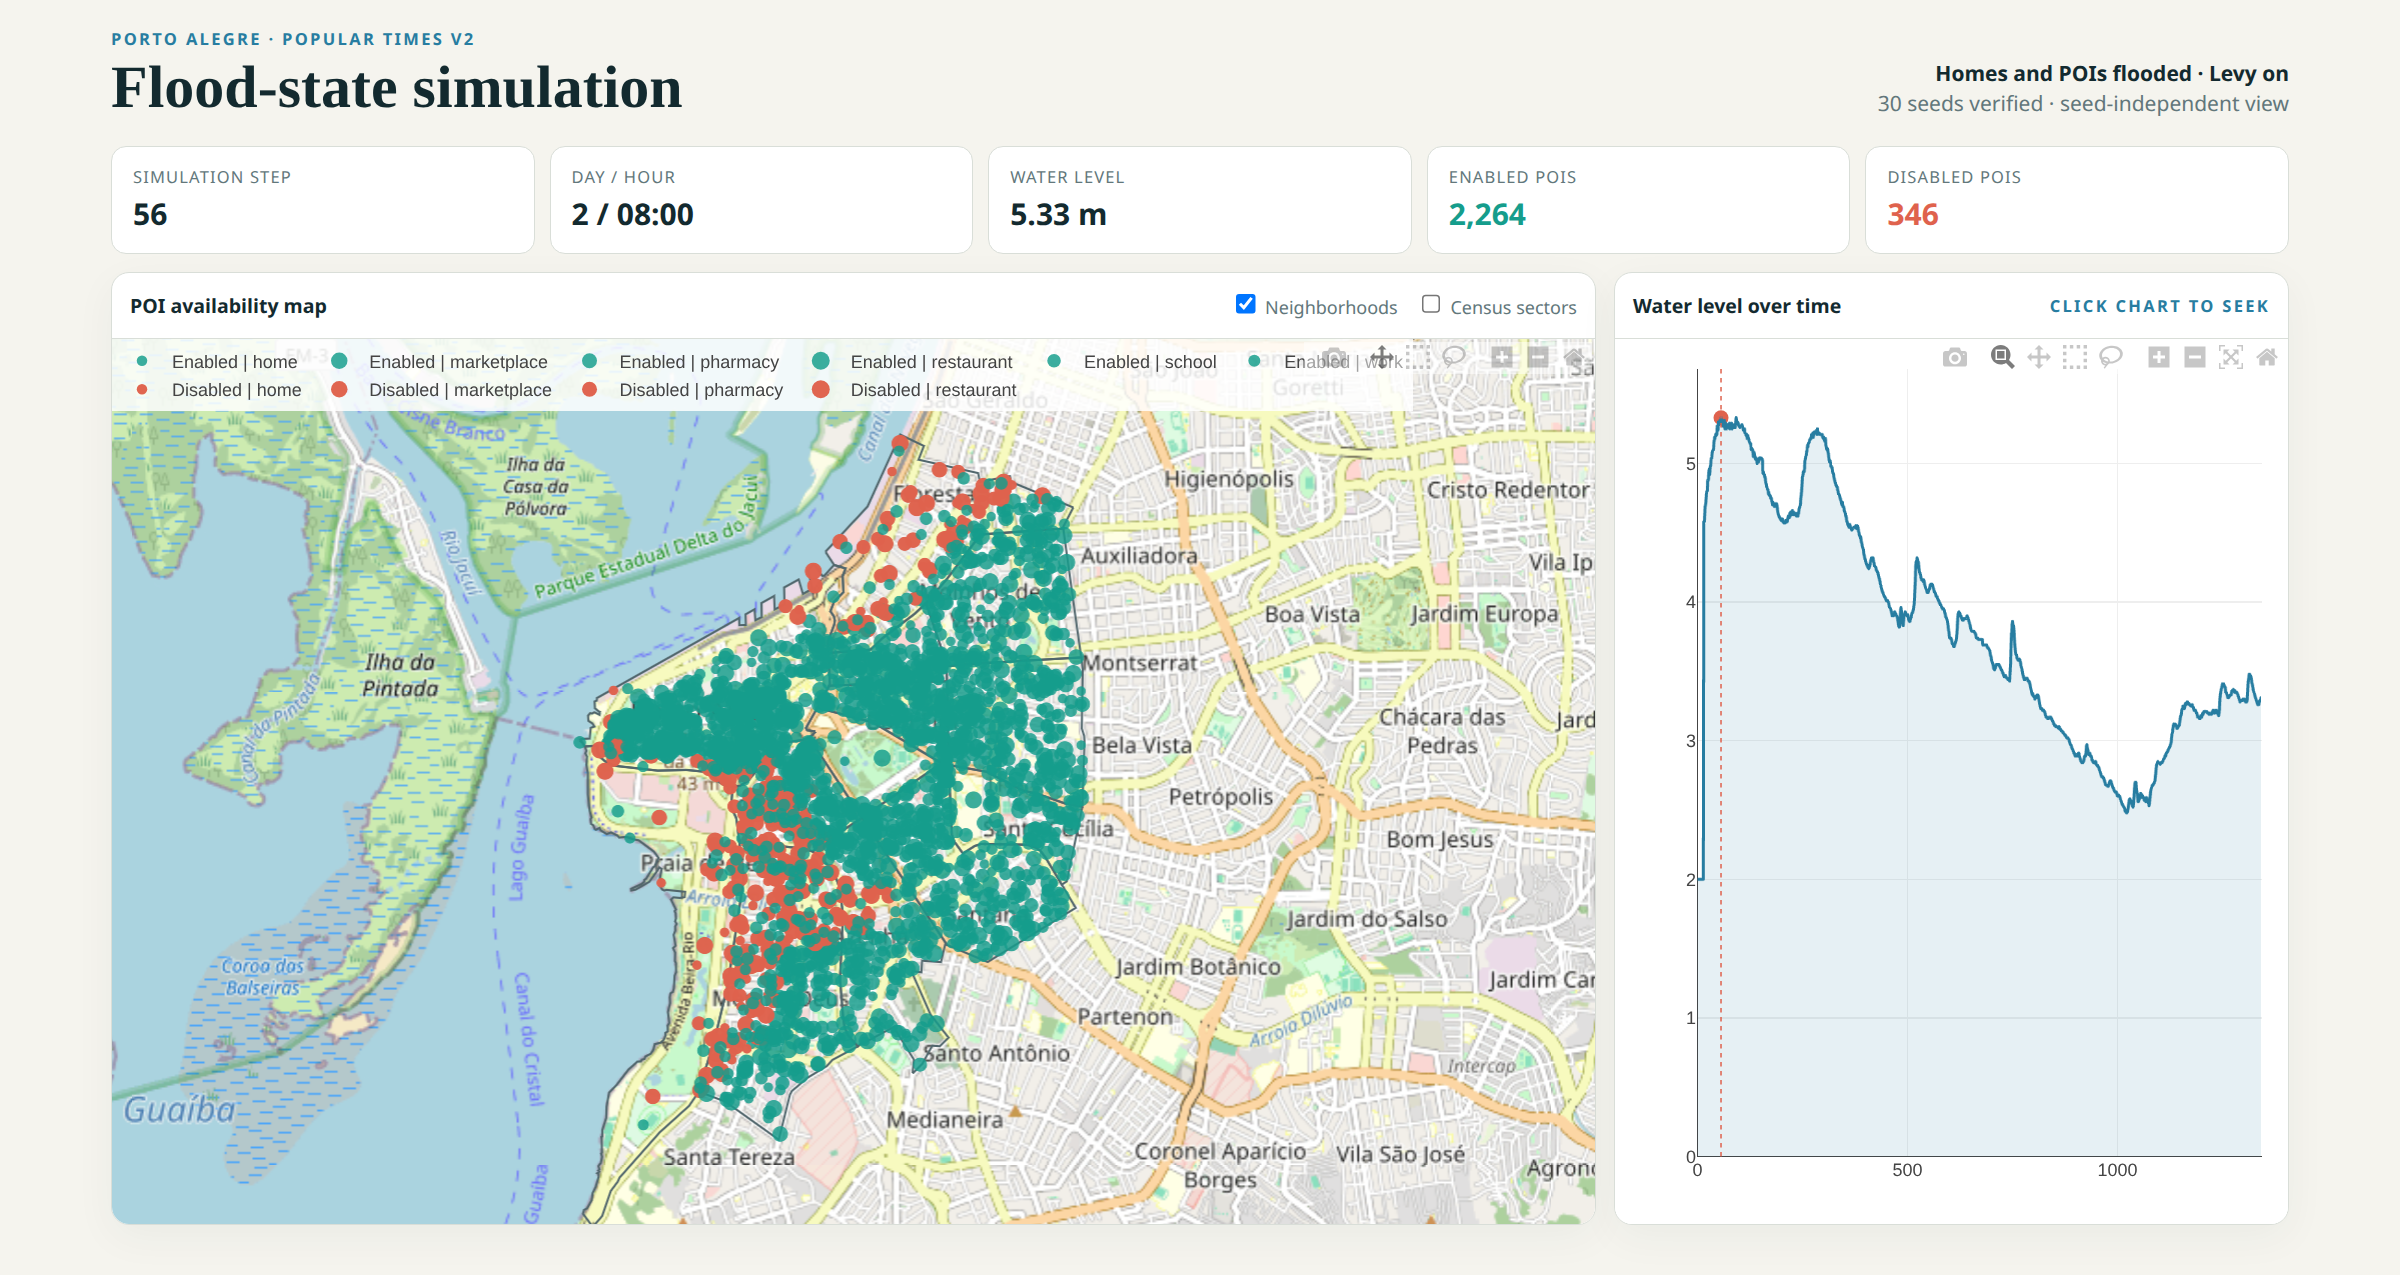
\includegraphics[width=0.99\textwidth]{fig/viz/flood_state_13_levy_both.png}
\caption{Flood-state snapshot for the reduced census-sector environment with L\'evy Walk enabled and the flood cause applied to home and activity POIs. At simulation step 56 (day 2, 08:00), the historical sequence reaches 5.33~m and makes 346 of the 2,610 modeled POIs unavailable. The map distinguishes available POIs from those carrying the flood disable cause.}
\label{fig:flood_state_visualization}
\end{figure}

\subsubsection{Shelter Locations and Capacities}

The shelter experiments examine whether populations displaced from flood-exposed areas can be redistributed to available emergency accommodation under spatial and capacity constraints. Their inputs therefore describe both the locations of shelters and the number of additional residents that each shelter can receive.

The geographic coordinates, capacities, and occupancies of shelters were collected from the Abrigos RS website on May 15, 2024\footnote{Abrigos RS: \url{https://abrigosrs.org/}.}. The shelter coordinates were taken from the geographic information made available by the website. The collected input contains 128 tabular records with names, addresses, coordinates, neighborhoods, capacities, occupancies, and free-text observations. After filtering and treatment of missing values, we consider 104 shelters with a combined capacity of 12,519 people and an initial occupancy of 10,963.

The retained records are instantiated as POIs of type \textit{shelter}. Their identifiers, coordinates, reported capacities, and initial occupancies are stored through conventions for $\bm{\alpha}_i$ declared by the shelter plugin. Capacity and displacement parameters form $\bm{\theta}_{\Pi}$, while the handlers and hooks in $\mathcal{F}_{\Pi}$ and $\mathcal{H}_{\Pi}$ determine admission, denial, reallocation, and return behavior. These values therefore remain plugin-interpreted service state rather than universal fields with behavior fixed by the core environment.

Figure~\ref{fig:shelter_locations_status} presents the locations and reported initial occupancy status of shelters with available capacity and occupancy information. The map makes visible both the uneven spatial distribution of shelter capacity and the limited number of places available before any simulated evacuation occurs.

\begin{figure}[ht]
\centering
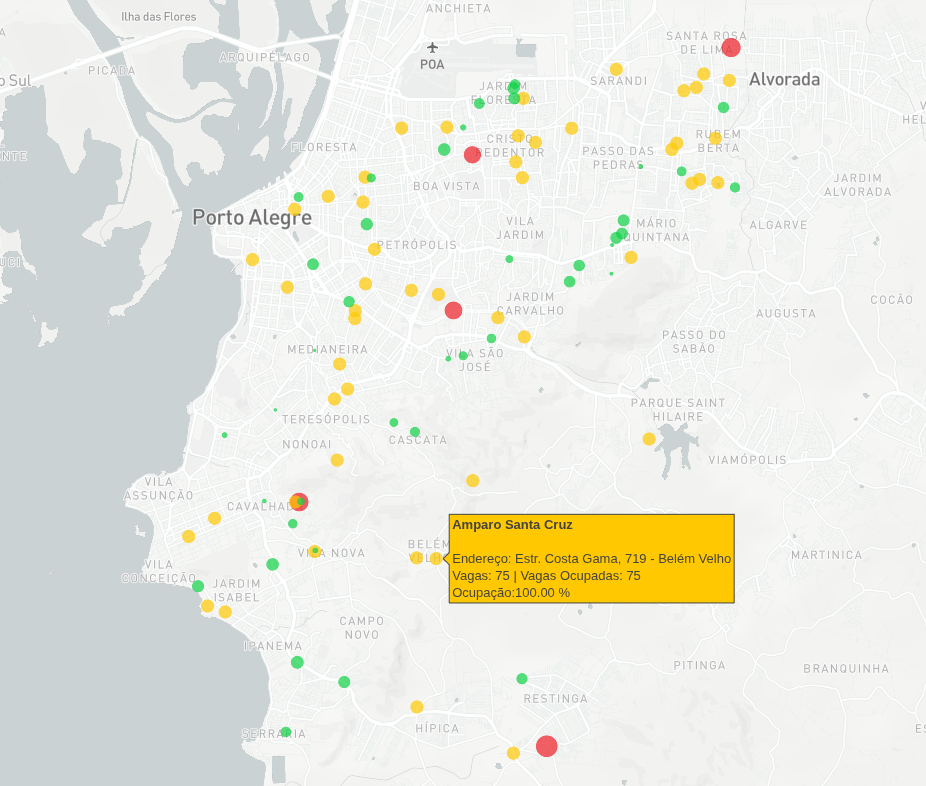
\includegraphics[width=0.85\textwidth]{fig/viz/shelters.png}
\caption{Shelter locations and reported initial occupancy status in Porto Alegre. Green markers identify shelters with available places, yellow markers identify shelters at their recorded capacity, and red markers identify shelters whose recorded occupancy exceeds their recorded capacity. Marker size is proportional to recorded capacity. The highlighted Amparo Santa Cruz record illustrates the address, capacity, occupied places, and utilization reported for an individual shelter.}
\label{fig:shelter_locations_status}
\end{figure}

\subsection{Health-Service Inputs: Dialysis}
\label{sec:infrastructure_input_data}

The health-service experiments examine access to recurring, capacity-constrained dialysis treatment under changes in demand and service availability. In addition to direct clinic disruptions, the scenarios represent dependencies on supporting water infrastructure, allowing failures at water-treatment facilities to indirectly affect access to dialysis services.

The dialysis environments represent Porto Alegre water-treatment stations (Estações de Tratamento de Água, ETAs) as POIs of type \textit{water source} and dialysis facilities as POIs of type \textit{dialysis clinic}. The complete overlay contains six ETAs and 12 clinics. ETA locations and the assignment of neighborhoods to water-supply systems were derived from maps and descriptions published by the Municipal Department of Water and Sewage (DMAE) and from a May 2024 account of water distribution and interconnections between the city's systems\footnote{DMAE water-system information: \url{https://prefeitura.poa.br/dmae/informacoes-agua}. GZH description of water distribution by neighborhood and connections between systems: \url{https://bit.ly/3TOMmnY}.}. The six ETAs reported by DMAE correspond to the six treatment stations represented in the complete environment.

Dialysis-clinic locations and clinic-to-water-source relations were provided by colleagues of the author based on their domain knowledge and the water-supply maps and sources cited above. Each clinic-to-source relation is represented by a dependency constraint in $D_i$, whereas names, coordinates, and external identifiers are stored in the relevant POI attribute mappings. Clinic opening and closing times and hourly treatment capacities are synthetic scenario parameters included in $\bm{\theta}_{\Pi}$.

The dialysis plugin uses $\Delta\Sigma_{\Pi}$ to declare the traceable characteristics required to represent patient selection, treatment frequency, due dates, status, origin, and treatment time. Its registered handler and time-step hook in $\mathcal{F}_{\Pi}$ and $\mathcal{H}_{\Pi}$ generate recurring demand, apply clinic capacity and schedule constraints, and perform treatment and return transitions.

The dialysis stress tests combine these service inputs with independent mechanisms for changing POI availability. A scheduled water-source outage adds its own direct cause to the source's $C_i(t)$, while flood exposure adds the distinct \textit{flood} cause to each affected source or clinic. The constraints $D_i$ then propagate source unavailability to dependent clinics. Removing one direct cause cannot restore a POI while another cause or an unsatisfied dependency remains. Synthetic sudden-rise water-level sequences, including transitions to 9.3~m and 10.1~m, are used as controlled stress conditions rather than observed hydrographs.


\section{Input Provenance and Interpretation}
\label{sec:input_provenance_summary}

Because the experiments combine externally sourced data, derived spatial attributes, and scenario-defined parameters, their provenance must be considered when interpreting the results. This distinction is particularly important when controlled experimental inputs are used to test model behavior rather than to reproduce observed conditions in Porto Alegre.
Table~\ref{tbl:simulation_data_provenance} summarizes the role and sources of the principal data families in the same general order in which they are introduced above.

\begin{table}[ht]
\centering
\footnotesize
\setlength{\tabcolsep}{4pt}
\caption{Provenance and interpretive status of the principal environment and scenario-input families.}
\label{tbl:simulation_data_provenance}
\begin{tabularx}{\linewidth}{@{}p{3.5cm}p{6.2cm}X@{}}
\toprule
\textbf{Data family} & \textbf{Documented basis} & \textbf{Interpretive status} \\
\midrule

Neighborhood geometry and POIs
& City Hall boundaries and OpenStreetMap amenities
& Externally sourced spatial data used to construct the neighborhood-level environment. \\

Neighborhood population
& IBGE, ObservaPOA, and PROCEMPA
& Externally sourced demographic data used to initialize the population represented in each neighborhood. \\

Census-sector environments
& IBGE 2022 geometries and aggregates
& Official census data spatially processed to construct the finer-grained population and POI representation. \\

L\'evy Walk parameters
& Scenario-defined behavioral and routine parameters
& They support controlled mobility comparisons and are not calibrated estimates of observed Porto Alegre trajectories. \\

Popular Times profiles
& Synthetic type-specific profiles generated from patterns observed in Google Maps Popular Times
& The profiles are scenario inputs rather than measured visitation data. \\

Large-scale event inputs
& Existing modeled event locations with scenario-defined event times and attendee requests
& The request of 500,000 attendees per event is a stress parameter rather than an observed attendance value. \\

Contagion parameters
& Reported $R_0$ values from studies of COVID-19 transmission in Brazil; remaining epidemic and restriction parameters configured by scenario
& The experiments provide controlled comparisons rather than calibrated epidemiological forecasts. \\

Vaccination quantities
& Applied-dose series from the Rio Grande do Sul vaccination dashboard
& Observed daily vaccination quantities; doses are distributed among modeled regions in proportion to their populations.\\

Flood thresholds and exposure
& Climate Central simulated water-level map evaluated at POI coordinates
& Derived exposure attributes representing the minimum modeled water level at which each location becomes inundated.\\

Water-level
& Public Power BI records from May--June 2024 plus synthetic stress sequences
& Historical observations are used for flood-mobility scenarios, while synthetic sequences are used for controlled stress experiments.\\

Shelters
& Abrigos RS snapshot collected on May 15, 2024
& Historical snapshot of shelter locations, capacities, and occupancies; the original source is no longer available online. \\

ETAs and dialysis clinics
& DMAE and GZH water-system information; clinic data and dependency definitions supplied by author colleagues
& Infrastructure locations and dependencies provide the scenario topology, while clinic schedules and hourly treatment capacities are synthetic experimental parameters. \\
\bottomrule
\end{tabularx}
\end{table}

Across the following results, externally sourced coordinates, population quantities, and capacities provide geographic and operational context, while behavioral parameters, demand volumes, failures, environmental conditions, and policy responses define the comparisons being tested. Consequently, uncertainty in the source data and uncertainty due to stochastic simulation represent different aspects of the experiments.
